\documentclass{ltjsarticle}
\usepackage{amsmath}
\usepackage{amssymb}
\usepackage{ascmac}
\usepackage[dvipdfmx]{graphicx}
\usepackage[colorlinks=true, allcolors=blue]{hyperref}
\usepackage{fancybox}
\usepackage{tikz}
\usepackage{subcaption}
\usetikzlibrary{shapes,arrows}

\begin{document}

\title{深層学習 day3}
\author{秋葉洋哉}
\maketitle

\section{day3 : 再帰型ニューラルネットワーク(RNN)}
\subsection{概要}
RNNは、時系列データを扱う際に有効なニューラルネットワークである。
時系列データとは、時間的順序を追って一定間隔毎に観測され、相互に統計的依存関係が認められるようなデータの系列のことである。
例えば、音声データ、テキストデータ、株価データなどが挙げられる。
(テキストデータが時系列データとなるのは、単語の並び順によって文章が構築されるためである。)
RNNは、時系列データの特徴を捉えるために、中間層の出力が次の時刻の入力として用いられる。

\subsection{RNNにおける順伝搬}
以降では、RNNの基本的な構造について説明するため、系列$\mathbf{x_1}, \mathbf{x_2}, \cdots$ をRNNに順番に入力したときに、対応する出力$\mathbf{y_1}, \mathbf{y_2}, \cdots$ を得ることを考える。
まず、入力層・中間層・出力層の各ユニットのインデックスを$i, j, k$とする。そして、時刻$t$における中間層ユニットへの出力を$\mathbf{u^t} = (u^t_j)$と$\mathbf{z^t} = (z^t_j)$、出力層のユニットへの出力を$\mathbf{v^t} = (v^t_k)$ と $\mathbf{y_t}=(y^t_k)$とする。入力層と中間層間の重みを$W^{\text{(in)}} = W^{\text{(in)}}_{ji}$、中間層から中間層への重みを$W = (W_{jj'})$、中間層と出力層間の重みを$W^{\text{(out)}} = W^{\text{(out)}}_{kj}$とする。

この時、時刻$t$における中間層$j$ユニットへの出力$u^t_j$は、以下のように表される。
\begin{align}
  u^t_j = \sum_{i} W^{\text{(in)}}_{ji}x^t_i + \sum_{j'} W_{jj'}z^{t-1}_{j'}
\end{align}
これは、時刻$t$における中間層の各ユニットへの入力が、入力層からの入力と、前の時刻$t-1$における中間層の出力からの入力の和であることを示している。ここでは、$W^{\text{(in)}}_{j0}$ をバイアスとして与えている。
以上の導出過程の概略図を図\ref{fig:RNN_forward}に示す。
\begin{figure}[htbp]
  \centering
  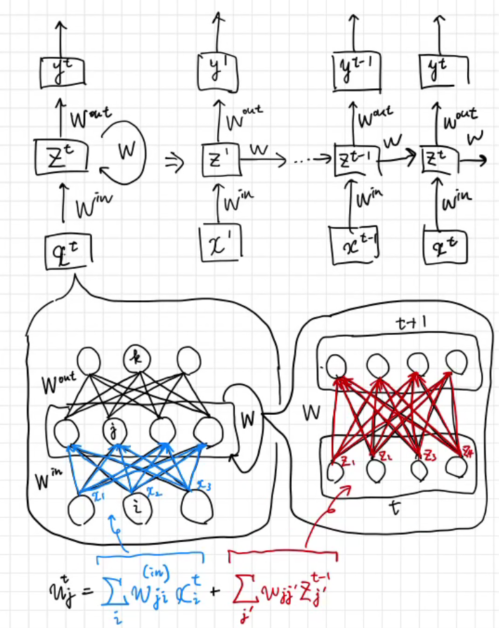
\includegraphics[width=10cm]{./capture/RNN.png}
  \caption{RNNにおける順伝搬の概略図}
  \label{fig:RNN_forward}
\end{figure}

活性化関数を$f(u^t_j)$とすると、中間層の出力$z^t_j$は、
\begin{align}
  z^t_j = f(u^t_j)
\end{align}
となる。これらをまとめると、時刻$t$における中間層の入力$\mathbf{u^t}$、出力$\mathbf{z^t}$、出力層の入力$\mathbf{v^t}$、出力$\mathbf{y^t}$は、
\begin{align}
  \mathbf{u^t} &= \mathbf{W^{\text{(in)}}}\mathbf{x^t} + \mathbf{Wz^{t-1}}\\
  \mathbf{z^t} &= f(\mathbf{W^{\text{(in)}}}\mathbf{x^t} + \mathbf{Wz^{t-1}})\\
  \mathbf{v^t} &= \mathbf{W^{\text{(out)}}}\mathbf{z^t} + c\\
  \mathbf{y^t} &= g(\mathbf{W^{\text{(out)}}}\mathbf{z^t} + c)
\end{align}
となる。ただし、$c$は出力層のバイアスである。また、$g$は出力層の活性化関数である。



\subsection{RNNにおける誤差逆伝播法}
RNNで誤差逆伝播法を用いて重みを更新する際には、RTRL(Real Time Recurrent Learning)やBPTT(Back Propagation Through Time)といった手法が用いられる。前者はメモリ効率が良く、後者は計算効率が良いという特徴がある。ここではBPTTについて説明する。

RNNでは、時刻$t$の中間層$j$の入力$u_j^t$を以下で表した。
\begin{align}
  u_j^t = \sum_i W_{ji}^{\text{(in)}}x_i^t + \sum_{j'} W_{jj'}z_{j'}^{t-1}
\end{align}
これは、時刻$t$における入力層からの入力$x_i^t$と、時刻$t-1$における中間層の出力$z_{j'}^{t-1}$からの入力に各重み成分を掛け合わせたの和としてあらわされている。

ここで、ニューラルネットワークの逆伝播では以下のように表せた。
\begin{align}
  \frac{\partial E}{\partial w_{ji}} &= \sum_t \frac{\partial E}{\partial u_j^t} \frac{\partial u_j^t}{\partial w_{ji}}\\
  &= \sum_t \delta_j^t z_i^t
\end{align}
ただし、$\delta_j^t$は中間層$j$の誤差であり、以下のように表される。
\begin{align}
  \delta_j = \frac{\partial E}{\partial u_j} = \frac{\partial E}{\partial z_j} \frac{\partial z_j}{\partial u_j}
\end{align}

RNNにおける$\delta_j^t$は、時刻$t$における出力層$k$の入力$v_k^t$と、時刻$t+1$における中間層$j'$の入力$u_{j'}^{t+1}$に依存するため、以下のように表される。
\begin{align}
  \delta_j^t &= \frac{\partial E}{\partial u_j^t}\\
   &= \sum_k \frac{\partial E}{\partial v_k^t} \frac{\partial v_k^t}{\partial u_j^t} + \sum_{j'} \frac{\partial E}{\partial u_{j'}^{t+1}} \frac{\partial u_{j'}^{t+1}}{\partial u_j^t}
\end{align}
まず、前半部分は、以下のように展開できる。
\begin{align}
  \sum_k \frac{\partial E}{\partial v_k^t} \frac{\partial v_k^t}{\partial u_j^t} &= \sum_k \delta_k^t \frac{\partial v_k^t}{\partial u_j^t}\\
  &= \sum_k \delta_k^t \frac{\partial}{\partial u_j^t} \left( \sum_{j} W_{kj}^{\text{(out)}}z_{j}^t + c \right)\\
  &= \sum_k \delta_k^t W_{kj}^{\text{(out)}} \frac{\partial z_j^t}{\partial u_j^t}\\
  &= \sum_k \delta_k^t W_{kj}^{\text{(out)}} \frac{\partial g(u_j^t)}{\partial u_j^t}\\
  &= \sum_k \delta_k^t W_{kj}^{\text{(out)}} g'(u_j^t)
\end{align}

そして、後半部分は、以下のように展開できる。
\begin{align}
  \sum_{j'} \frac{\partial E}{\partial u_{j'}^{t+1}} \frac{\partial u_{j'}^{t+1}}{\partial u_j^t} &= \sum_{j'} \delta_{j'}^{t+1} \frac{\partial u_{j'}^{t+1}}{\partial u_j^t}\\
  &= \sum_{j'} \delta_{j'}^{t+1} \frac{\partial}{\partial u_j^t} \left( \sum_i W_{j'i}^{\text{(in)}}x_i^{t+1} + \sum_{j} W_{j'j}z_{j}^t \right)\\
  &= \sum_{j'} \delta_{j'}^{t+1} \frac{\partial}{\partial u_j^t} \left( \sum_i W_{j'i}^{\text{(in)}}x_i^{t+1} + \sum_{j} W_{j'j}f(u_j^t) \right)\\
  &= \sum_{j'} \delta_{j'}^{t+1} W_{j'j} f'(u_j^t)
\end{align}
よって、$\delta_j^t$は以下のように表される。
\begin{align}
  \delta_j^t =  \sum_k \delta_k^t W_{kj}^{\text{(out)}} g'(u_j^t) + \sum_{j'} \delta_{j'}^{t+1} W_{j'j} f'(u_j^t)
\end{align}

この結果を用いて、誤差関数を各重みで微分した値を導出できる。
\begin{align}
  \frac{\partial E}{\partial W_{ji}^{\text{(in)}}} &= \sum_{t=1}^T \frac{\partial E}{\partial u_j^t} \frac{\partial u_j^t}{\partial W_{ji}^{\text{(in)}}}\\
  &= \sum_{t=1}^T \delta_j^t x_i^t
\end{align}
\begin{align}
  \frac{\partial E}{\partial W_{jj'}} &= \sum_{t=1}^T \frac{\partial E}{\partial u_j^t} \frac{\partial u_j^t}{\partial W_{jj'}}\\
  &= \sum_{t=1}^T \delta_j^t z_{j'}^{t-1}
\end{align}
\begin{align}
  \frac{\partial E}{\partial W_{kj}^{\text{(out)}}} &= \sum_{t=1}^T \frac{\partial E}{\partial v_k^t} \frac{\partial v_k^t}{\partial W_{kj}^{\text{(out)}}}\\
  &= \sum_{t=1}^T \delta_k^t z_j^t
\end{align}

\begin{itembox}[l]{確認テスト}
  Q: 図\ref{fig:day3_07_1}について、$y_1$を、$x, z_0, z_1, W_{\text{(in)}}, W, W_{\text{(out)}}$を用いて数式で表せ。

  A: 以下導出の通り。ただし、$g$は活性化関数、$c$はバイアスである。
  \begin{align}
    y_1 &= \sum W_{\text{(out)}}z_1 + c\\
    &= \sum W_{\text{(out)}}g(\sum Wz_0 + \sum W^{\text{(in)}}x + c) + c
  \end{align}
\end{itembox}

\begin{figure}
  \centering
  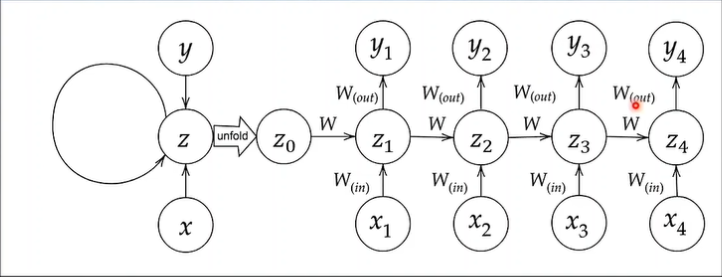
\includegraphics[width=10cm]{./capture/confirm_test/day3_07_1.png}
  \caption{}
  \label{fig:day3_07_1}
\end{figure}

\subsection{LSTM}
RNNは、時刻$t$における一つのニューラルネットワークを、$t=0$から$t=T$まで繰り返し適用するモデルである。
一つのニューラルネットワークでさえ、逆伝播において勾配消失問題について考える必要があるが、RNNでは、時刻が進むにしたがってより多くのニューラルネットワークを重ねていくため、逆伝播における勾配消失問題がより顕著になる。
また、逆に、時刻が進むにしたがって逆伝播における勾配が爆発する問題も発生する。
\begin{itembox}[l]{確認テスト}
  Q: RNNや深いモデルでは勾配の消失や爆発が起こる傾向がある。勾配爆発を防ぐために勾配のクリッピングという手法が使われることがある。具体的には勾配のノルムが閾値を超えたら、勾配のノルムを閾値に正規化するというものである。この関数を完成させなさい。

  A: 
  \begin{verbatim}
    def gradient_clipping(grad, threshold):
      norm = np.linalg.norm(grad) # 勾配のノルムを計算
      rate = threshold / norm
      if rate < 1:
        return grad * rate 
      return grad
  \end{verbatim}  

\end{itembox}

この問題を解決するために、LSTM(Long Short-Term Memory)が提案された。
図\ref{fig:LSTM}にLSTMの構造を示す。
\begin{figure}[htbp]
  \centering
  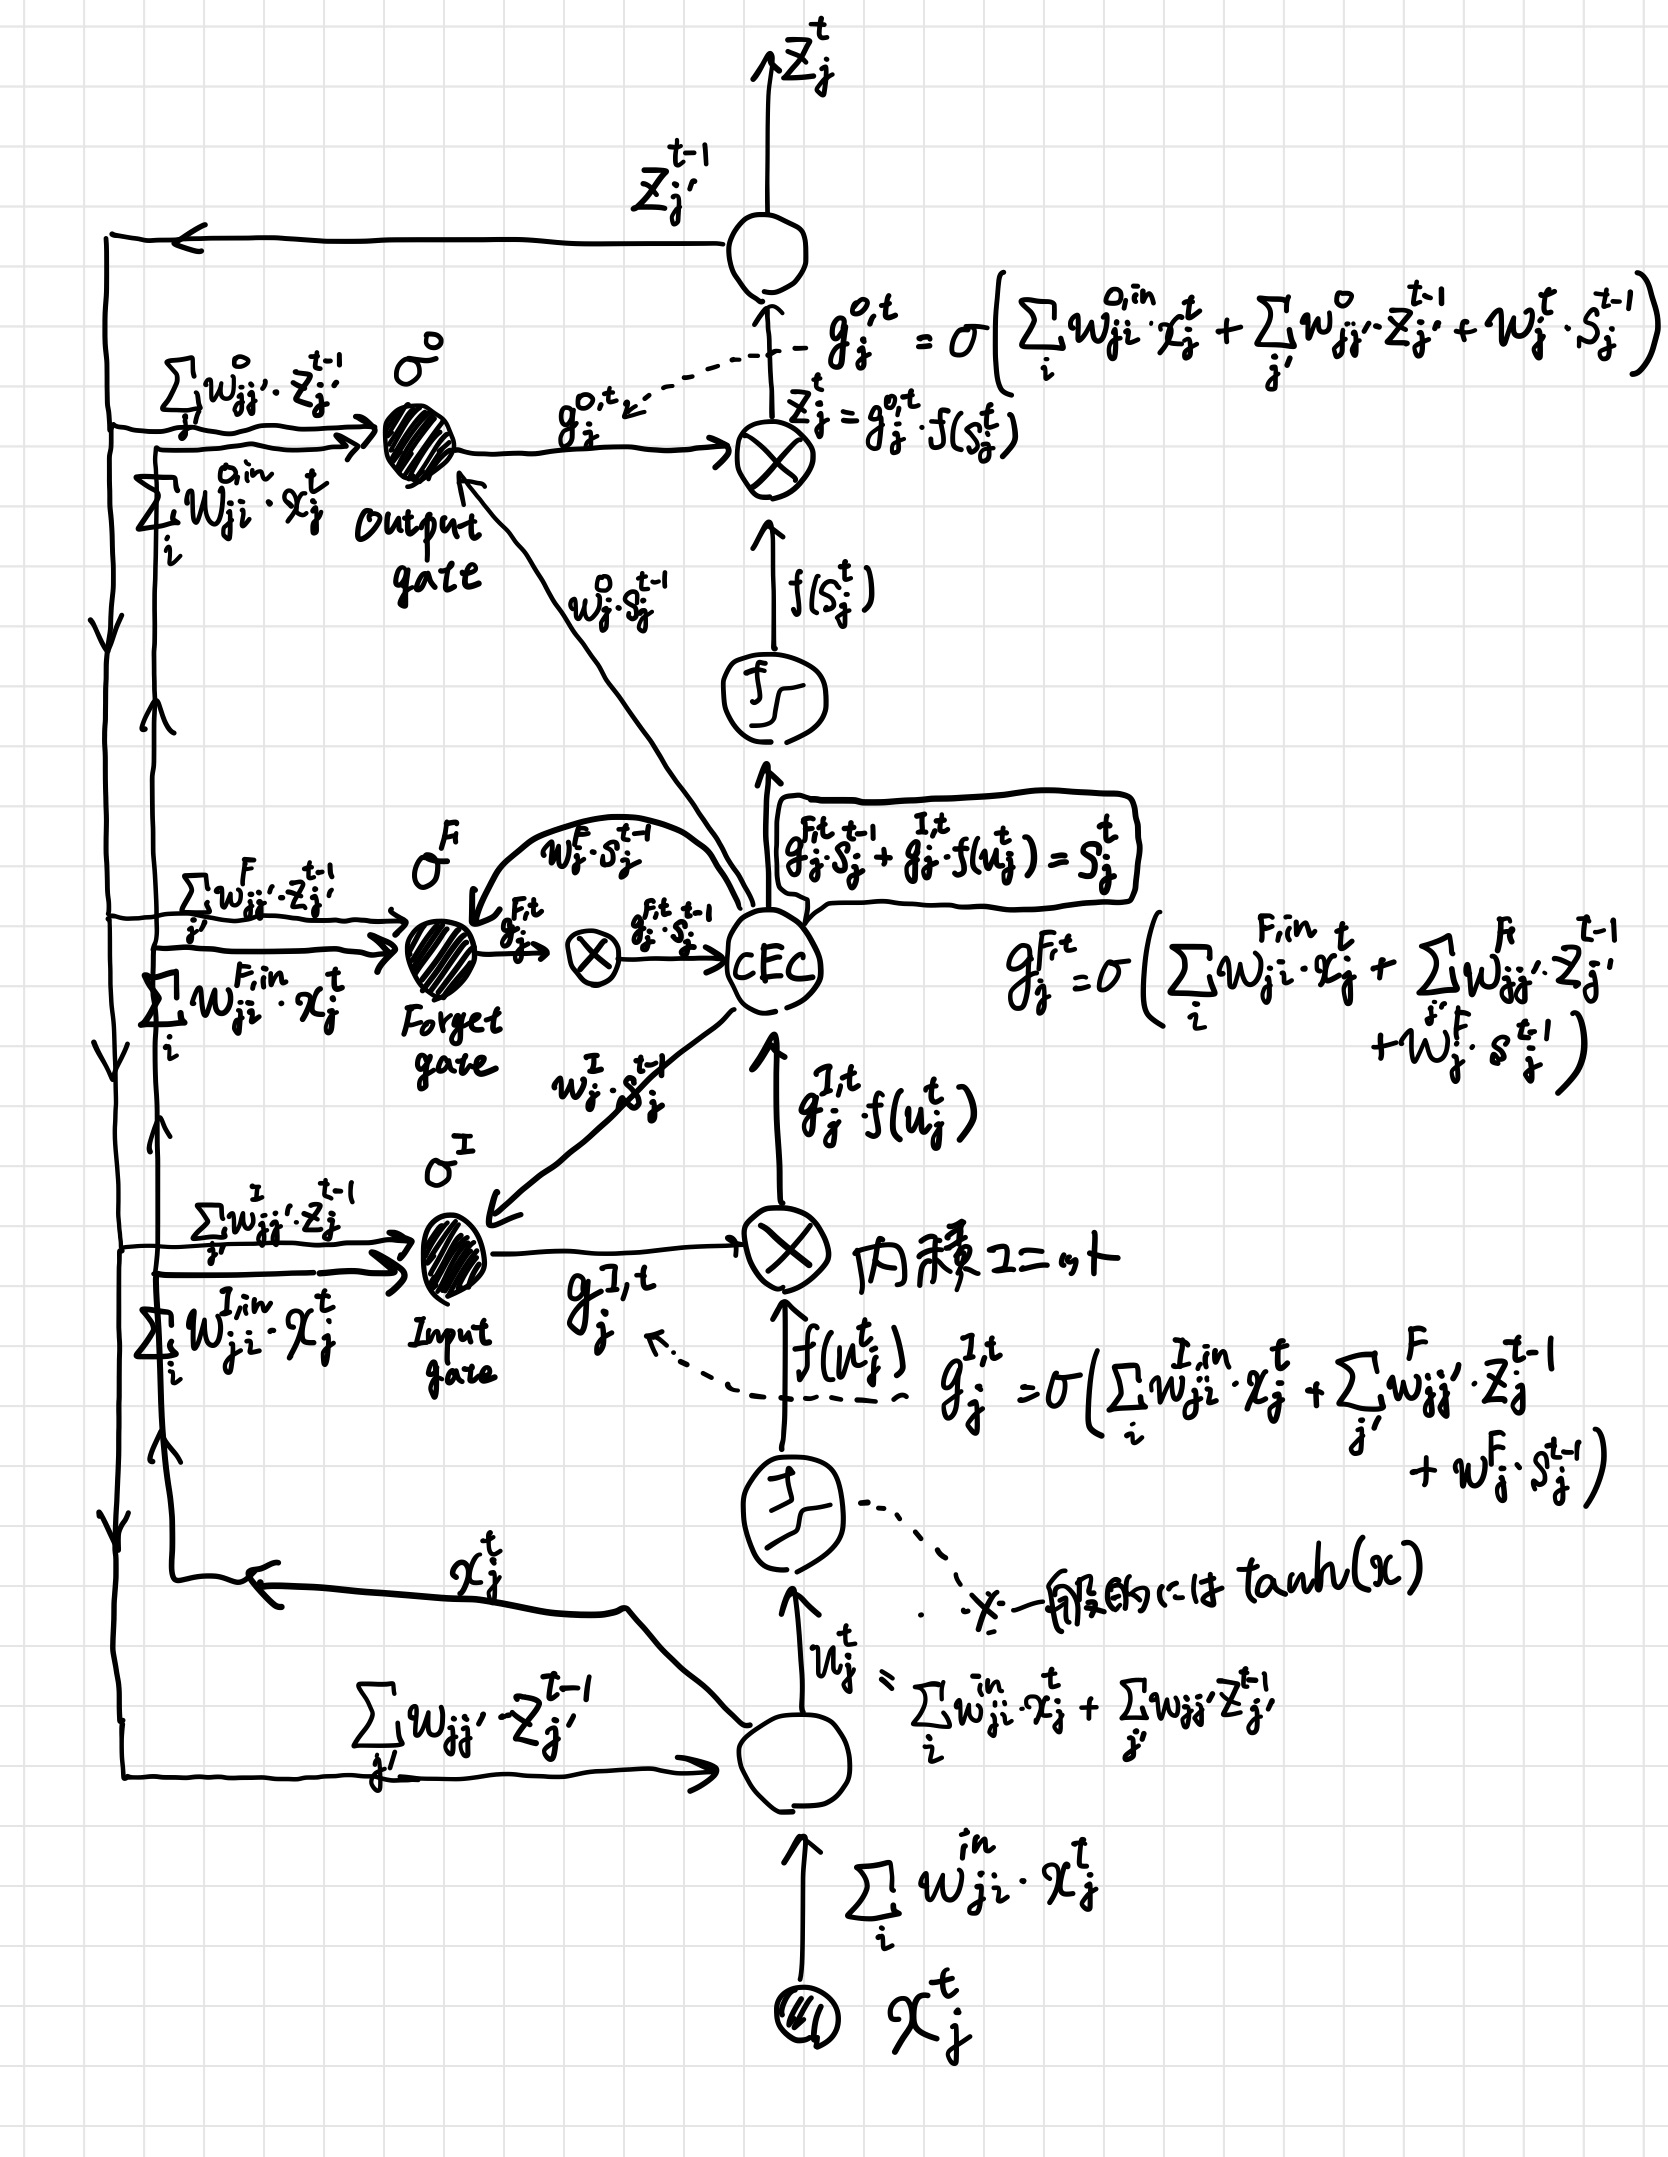
\includegraphics[width=13cm]{./capture/LSTM-33.jpg}
  \caption{LSTMの構造}
  \label{fig:LSTM}
\end{figure}

\newpage

図\ref{fig:LSTM}によれば、入力ゲート・出力ゲート・忘却ゲートの3つのゲートが存在し、入力・出力ゲートは層と層の間に設けられ、忘却ゲートはCEC(Constant Error Carrousel)と呼ばれる、過去の情報を保持するためのユニットとループ状態で接続されている。
\subsubsection{CEC}
CECは記憶を保持するためのユニットであり、学習機能有さない。学習の機能は各種ゲートによって制御され、CECに何を覚えさせるか、何を忘れさせるか、何を出力するかを制御する。
\subsubsection{入力ゲート}
入力ゲートでは、時刻$t$の入力$x_j^t$と、時刻$t-1$の出力$z_j^{t-1}$、そして、時刻$t-1$のCECの情報$s_j^{t-1}$の3つを入力として、新しい情報をCECに追加する。$x_j^t$, $z_j^{t-1}$, $s_j^{t-1}$に対してはそれぞれの別の重みが掛けられ、情報を重視する割合を調整する。この重みが学習によって最適化される。
\subsubsection{出力ゲート}
出力ゲートでは、時刻$t$の入力$x_j^t$と、時刻$t-1$の出力$z_j^{t-1}$、そして、時刻$t$CECの情報$s_j^{t}$の3つを入力として、最終的に出力する値の調整を行う。こちらにも割合を調整する重みが掛けられ、学習によって最適化される。
\subsubsection{忘却ゲート}
忘却ゲートでは、時刻$t$の入力$x_j^t$と、時刻$t-1$の出力$z_j^{t-1}$、そして、時刻$t-1$CECの情報$s_j^{t-1}$の3つを入力として、CECの情報をどれだけ忘れるかを調整する。もし、忘却ゲートが無かったら、過去の情報が無限に保持されることになる。このことは過去の情報がいらなくなった場合に、削除することができないことを意味する。忘却ゲートによって、過去の情報を必要な時に保持し、不要な時に削除することができる。これによって、勾配消失や勾配爆発を防ぐことができる。

\newpage

\begin{itembox}[l]{確認テスト}
  Q: 以下の文章をLSTMに入力し空欄に当てはまる単語を予測したいとする。文中の「とても」という言葉は空欄の予測において無くなっても影響を及ぼさないと考えられる。このような場合、どのゲートが作用すると考えられるか。
  \par
  「映画おもしろかったね。ところで、とてもお腹が空いたから何か\_\_\_\_\_。」

  A: 忘却ゲートが作用する。忘却ゲートによって過去の情報の有無を判断しているため、「とても」という単語の影響が少ないことを学習することができる。

  Q: LSTMの順伝搬を行うプログラムを書け。

  A: 以下に示す。
  \begin{verbatim}
    def lstm(x, prev_h, prev_c, W, U, b):
      """
      x: inputs, (batch_size, input_size)
      prev_h: previous output at time t-1, (batch_size, hidden_size)
      prev_c: previous cell state at time t-1, (batch_size, hidden_size)
      W: upwrad weights, (4*state_size, input_size)
      U: lateral weights, (4*state_size, hidden_size)
      b: biases, (4*state_size,)
      """

      # セルへの入力やゲートをまとめて計算し分割する
      a = np.dot(x, W.T) + np.dot(prev_h, U.T) + b
      a, ai, af, ao = np.split(a, 4, axis=1)

      # 各ゲートの計算
      ig = sigmoid(ai)
      fg = sigmoid(af)
      og = sigmoid(ao)

      # セルの値の計算
      c = fg * prev_c + ig * np.tanh(a) # 要素同士の積を求めるため、np.dotにはならないことに注意
      h = og * np.tanh(c)

      return h, c
  \end{verbatim}
\end{itembox}

\newpage

\subsection{GRU(Gated Recurrent Unit)}
LSTMでは、パラメータ数が多く、計算コストが高いという問題があった。この問題を解決するために、GRUが提案された。
GRUでは、LSTMの入力ゲートと忘却ゲートを「更新ゲート」として統合し、また、出力ゲートを廃止することで、パラメータ数を削減している。また、「リセットゲート」を導入することで、過去の情報をどれだけ保持するかを調整することができる。
CECへの入力値$\mathbf{u^t}$, CECの保持値$\mathbf{s^{t}}$, 出力$\mathbf{z^t}$は以下のように表される。
\begin{align}
  \label{eq:GRU1}
  \mathbf{u^t} &=\mathbf{W^{\text{(in)}}}\mathbf{x^t} + \mathbf{Wg}^{R,t} \odot z^{t-1}\\
  \mathbf{s^t} &= \mathbf{g}^{U,t} \odot \mathbf{s^t} + (1 - \mathbf{g}^{U,t}) \odot f(\mathbf{u^t})\\
  \mathbf{z^t} &= \mathbf{s^t}
\end{align}
ここで、$\odot$は要素積を表す。また、$\mathbf{g}^{R,t}$はリセットゲート、$\mathbf{g}^{U,t}$は更新ゲートの出力値で、
\begin{align}
  \mathbf{g}^{R,t} &= \sigma(\mathbf{W^R}\mathbf{x^t} + \mathbf{U^R}\mathbf{z^{t-1}})\\
  \mathbf{g}^{U,t} &= \sigma(\mathbf{W^U}\mathbf{x^t} + \mathbf{U^U}\mathbf{z^{t-1}})
\end{align}
と表される。$\sigma$はシグモイド関数である。
式\eqref{eq:GRU1}の右辺第二項の$\mathbf{g}^{R,t}$が無かった時、更新ゲートの値が0であった場合に、過去の状態が常に同じ割合($\mathbf{Wz^{t-1}}$)で現在に伝播されてしまうが、リセットゲートを導入することで、忘却ゲートのように過去の情報をどれだけ保持するかを調整することができる。

\subsection{双方向RNN}
双方向RNNは、時系列データを前方向と後方向の2つのRNNで処理し、それぞれの出力を結合することで、より正確な予測を行うことができる。文章の推敲や、機械翻訳などで利用される。
双方向RNNのPythonコードを以下に示す。
\begin{itembox}[l]{}
\begin{verbatim}
  import numpy as np

  def bidriectinoal_rnn(xs, W_f, U_f, W_b, U_b, V):
  """
  W_f, U_f : forward rnn weights, (hidden_size, input_size)
  W_b, U_b : backward rnn weights, (hidden_size, input_size)
  V: output weights, (output_size, hidden_size)
  """

    xs_f = np.zeros_like(xs)
    xs_b = np.zeros_like(xs)
    for i , x in enumerate
      xs_f[i] = x
      xs_b[i] = x[::-1]
    hs_f = forward_rnn(xs_f, W_f, U_f)
    hs_b = forward_rnn(xs_b, W_b, U_b)
    hs = [np.concatenate([h_f, h_b[::-1]], axis=1) for h_f, h_b in zip(hs_f, hs_b)]
    ys = hs.dot(V.T)
    return ys
\end{verbatim}
\end{itembox}
ここで、numpyのconcatenateは、配列を結合する関数である。具体的には、axis=0の場合、縦方向に結合し、axis=1の場合、横方向に結合する。そのあとのzip関数は、複数のリストを同時にループ処理するための関数である。こうすることで、過去と未来の情報を無くすこと無く、演算することができる。


\subsection{自己回帰モデル}
自己回帰モデルは、時系列データを入力し、その出力を次の時刻の入力として再帰的に処理するモデルである。RNNは、自己回帰モデルの一種である。
\begin{align}
  \mathbf{x}^t = \phi_0 + \sum_{i=t-\rho}^{t-1} \phi_i \mathbf{x}^i + \epsilon^t
\end{align}
ここで、$\phi_0$は定数項、$\phi_i$は係数、$\epsilon^t$はノイズである。この式は、時刻$t$における入力$\mathbf{x}^t$が、過去の入力$\mathbf{x}^{t-1}, \mathbf{x}^{t-2}, \cdots$に依存していることを示している。

\subsection{Seq2Seq}
Seq2Seqは、時系列データを入力として、長さの異なる時系列データを出力するモデルである。機械翻訳や対話モデルなどで利用される。
Seq2Seqの構造は、図\ref{fig:Seq2Seq}のようになる。
\begin{figure}[htbp]
  \centering
  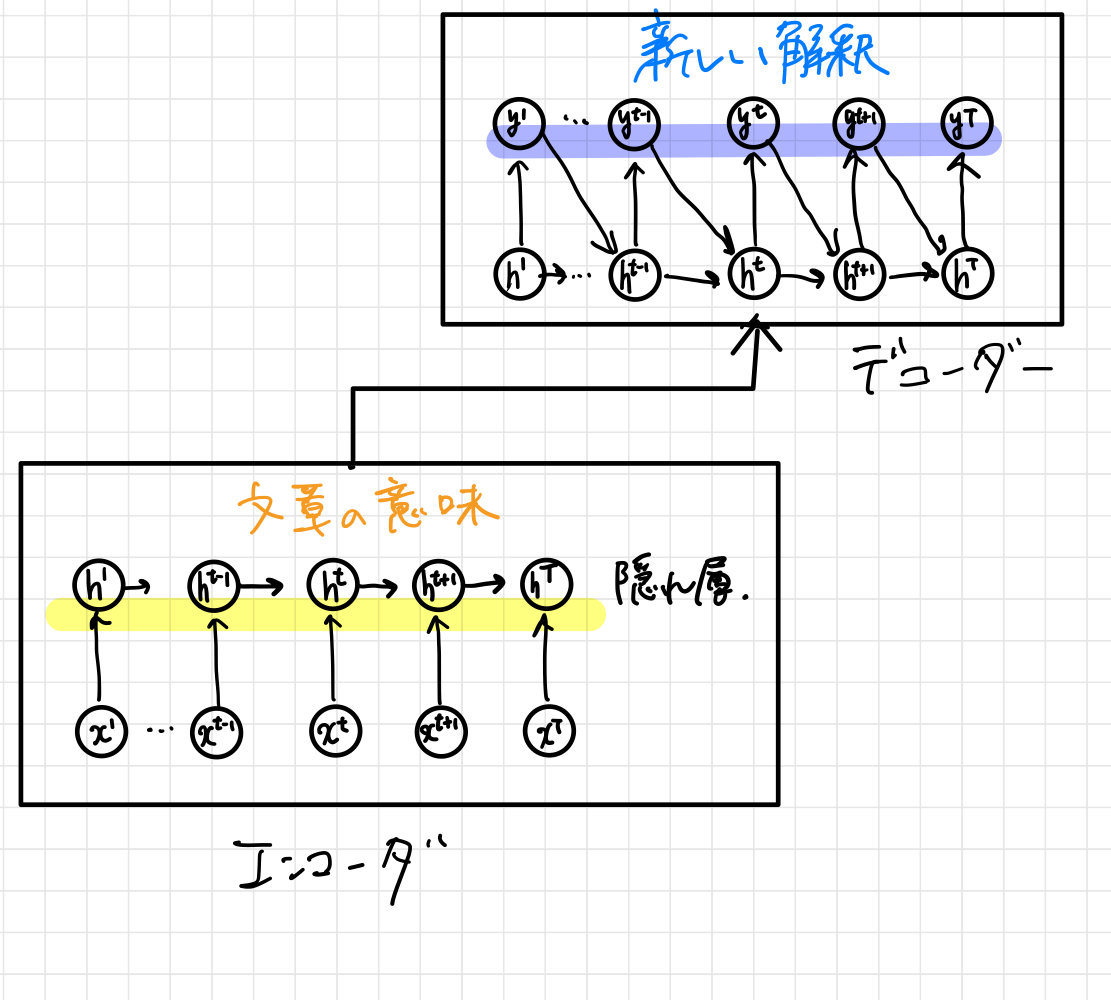
\includegraphics[width=13cm]{./capture/Seq2Seq.png}
  \caption{Seq2Seqの構造}
  \label{fig:Seq2Seq}
\end{figure}

Seq2Seqは、エンコーダとデコーダから構成される。エンコーダは、入力データを受け取り、中間層の出力をデコーダに渡す。デコーダは、エンコーダから受け取った中間層の出力を元に、出力データを生成する。エンコーダとデコーダは、LSTMやGRUなどのRNNを用いて構築される。

\subsubsection{Encoder RNN}
エンコーダでは、主に、Taking, Embedding, RNNの3つの処理を行う。
Takingでは、ユーザーがインプットしたデータを単語毎に分割する。
\par
Embeddingでは、分割した単語をベクトルに変換する。例えば英語なら、英単語のうち代表的なものを$K$語選び、これを 1-of-$K$符号化する。これをEmbedding Matrixと呼ぶ。その後、入力に対して各単語に対応するベクトルを生成する。このベクトルは、似た単語の意味は似た配列となるように機械学習によって生成される。
\par
RNNでは、Embeddingで生成されたベクトルを入力として受け取る。例えば、文章の途中を隠して単語を予測したり、後に続く文章を生成したりすることができる。

\subsubsection{Decoder RNN}
Encoderの内部状態を入力して、出力を生成する。この時、用いるEmbedding Matrixは、必ずしもEncoderで利用した$K$語の単語である必要はなく、異なる言語のEmbedding Matrixを用いることもできる。こうすることで、異なる言語間での翻訳が可能となる。

\subsubsection{HRED}
HRED(Hierarchical Recurrent Encoder-Decoder)は、Seq2Seqの拡張モデルである。Seq2Seqでは、文脈を考慮した応答ができないという問題があったが、HREDでは、文脈を考慮した応答が可能となる。
Seq2Seqにおけるエンコーダの中間層の出力を、さらに過去のエンコーダ出力とRNNと繋いで処理する。この、会話コンテキスト全体を表すベクトルをContext RNNと呼ぶ。
\par
ただし、HREDは同じコンテキストが与えられた場合に、同様の出力になってしまったり、短い返答を学んでしまう問題があった。この問題を解決するために、VHRED(Variational Hierarchical Recurrent Encoder-Decoder)が提案された。VHREDは、HREDにVAE(Variational Auto-Encoder)を組み合わせたモデルである。VAEは、データの生成過程を確率モデルとして表現し、データの生成過程を学習するモデルである。VHREDは、HREDの中間層の出力をVAEの入力として、文脈を考慮した応答を生成する。

\subsection{VAE(Variational Auto-Encoder)}
\subsubsection{オートエンコーダ}
オートエンコーダーは、教師無し学習を用いて、入力と出力が同じ値になるように、エンコーダとデコーダを作成していく、教師無し学習の一つである。
入力と潜在変数の間にはエンコーダが、出力と潜在変数の間にはデコーダが存在する。エンコーダによって入力データを次元削減し、特徴を抽出する。デコーダによって、次元削減されたデータを元の次元に戻す。この時、入力と出力が同じになるように学習を行う。

\subsection{word2vec}
\subsubsection{概要}
word2vecは、単語をベクトルに変換する手法である。word2vecはたった2層のニューラルネットワークで構成されているが、単語の意味をベクトル化することができる。
word2vecには、CBOW(Continuous Bag of Words)とSkip-gramの2つの手法がある。
CBOWは、周囲の単語から中央の単語を予測するモデルである。Skip-gramは、中央の単語から周囲の単語を予測するモデルである。
word2vecは、単語の意味をベクトル化することができるため、自然言語処理の分野で広く利用されている。
\par
word2vecで巨大なコーパスを扱う場合、通常の多クラス分類(100万語の中から1語を取り出す方法)を行うと計算速度が問題となる。この問題を解決するために、負例サンプリング (negative sampling)という手法を用いて、損失関数の計算を高速化することができる。
\par
通常のCBOW及びSkip-gramにおける出力層では、すべての語彙を対象としてソフトマックス関数と交差エントロピー誤差関数の計算を行う。つまり、語彙数が100万、中間層の数が100の場合、1回の学習で要する計算量は100万×100×2(順・逆)となる。
\par
しかし、負例サンプリングを用いた場合の出力層では、1個の正例と$k$(ハイパーパラメータ)個の負例の語彙のみを対象として、シグモイド関数と交差エントロピー誤差関数の計算を行う。つまり、出力層のニューロン数は$1+k$となる。
$k$の設定は、小さなデータセットなら$k=2\sim5$、大きなデータセットなら$k=5\sim20$程度が適している。

\subsubsection{Skip-gram}
Skip-gramでは、ある単語を入力したとき、その周辺にどのような単語が表れやすいかを予測する。例えば以下のような例文があったとする。
\begin{itembox}[l]{}
    I want to eat an apple every day.
\end{itembox}
eatを入力としたとき、周辺にはapple や orangeといった単語が表れる確率が高く予測し、tank や networkといった単語が表れる確率が低いと予測するのが、Skip-gramの手法である。この出現確率を、ボキャブラリ内のすべてに対して計算することで、各単語のベクトルを生成する。このベクトルは、単語の意味を表すベクトルであり、単語ベクトルと呼ばれる。
\par
Skip-gramは教師あり学習である。入力として、eatのような単語を与え、正解データとしてapple, orangeなどの周辺の単語を与える。学習が進むと、入力単語に対して周辺の単語が出現する確率が高くなるようになる。
\begin{figure}[htbp]
  \centering
  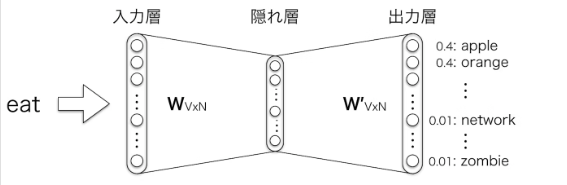
\includegraphics[width=10cm]{./capture/Skip-gram_1.png}
  \caption{Skip-gramでは周辺の単語の出現確率を予測する。(https://qiita.com/Hironsan/items/11b388575a058dc8a46a より引用)}
  \label{fig:Skip-gram_1}
\end{figure}

\paragraph{入力層}
Skip-Gramの入力層では、ボキャブラリ内の単語を1-of-$V$符号化する。例えば、ボキャブラリがI, want, to, eat, an, apple, every, dayの8単語で構成されている場合、eatを入力としたとき、入力層は以下のようになる。
\begin{align}
  \begin{pmatrix}
    0\\
    0\\
    0\\
    1\\
    0\\
    0\\
    0\\
    0
  \end{pmatrix}
\end{align}
これは、eatが4番目の単語であることを示している。

\paragraph{中間層}
中間層では、入力層の単語をベクトルに変換する。このベクトルは、各単語の意味を表すベクトルであり、単語ベクトルと呼ぶ。例えば、入力層のベクトルが10000次元(10000単語のボキャブラリ)、中間層のレイヤー数を300とすると、各単語ベクトルは300次元のベクトルとなる。この単語ベクトルは、ある単語一つに対する、他の9999単語の出現確率を予測する重み行列である。

\begin{figure}[htbp]
  \centering
  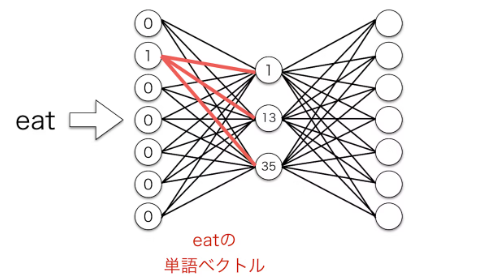
\includegraphics[width=10cm]{./capture/Skip-gram_2.png}
  \caption{この例では、eatという単語だけを入力で与えた時に抽出される重みは1, 13, 35となる。 (https://qiita.com/Hironsan/items/11b388575a058dc8a46a より引用)}
  \label{fig:Skip-gram_2}
\end{figure}

\paragraph{出力層}
出力層では、中間層の1×300のベクトルを、出力層との間の単語ベクトルとの内積を計算し、出力層の単語の出現確率を計算する。出力層に入力された値は、ソフトマックス関数を通して、確率に変換される。

\begin{figure}[htbp]
  \centering
  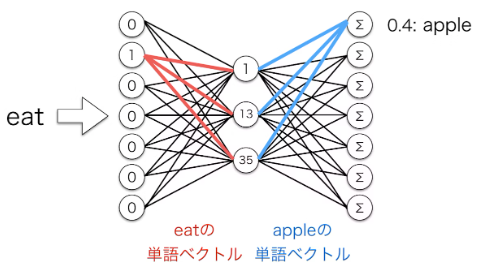
\includegraphics[width=10cm]{./capture/Skip-gram_3.png}
  \caption{eatを与えた時にappleを予測する場合に使われる単語ベクトル (赤・青のルート) (https://qiita.com/Hironsan/items/11b388575a058dc8a46a より引用)}
  \label{fig:Skip-gram_3}
\end{figure}

\subsubsection{CBOW(Continuous Bag of Words)}
CBOWは、Skip-gramとは逆に周囲の単語から中央の単語を予測するモデルである。CBOWは、Skip-gramよりも学習が速いという特徴がある。入力は周辺語、出力は中央語である。

CBOWもSkip-gramも、同様に入力層側の重み$W_{\text{in}}$と、出力層側の重み$W_{\text{out}}$をパラメータとして持つが、一般に$W_{\text{in}}$を単語埋め込み行列として利用する。


\subsection{Attention Mechanism (注意機構)}
Attention Mechanismは、Seq2Seqの問題点である、長い文章を処理する際に、過去の情報が失われてしまう問題を解決するために提案された。Attention Mechanismは、入力データの各単語に重みを付け、重要な単語に大きな重みを付けることで、過去の情報を保持することができる。Attention Mechanismにはいくつかの種類があり、その中でも、自己注意機構(Self-Attention Mechanism)は、先ほどのSkip-gramと同様に、単語のベクトルを生成する手法であり、Transformerと呼ばれるモデルに用いられる。

\subsection{Spoken Degit}
Spoken Degitは、音声データを入力として、0から9までの数字を出力するモデルである。音声データは、MFCC(Mel-Frequency Cepstral Coefficients)と呼ばれる特徴量に変換され、RNNに入力される。RNNは、音声データを時系列データとして処理し、出力として0から9までの数字を出力する。

TensorFlowでSpoken Degitを実装する場合、
\begin{itembox}[l]{}
\begin{verbatim}
  dataset_train, dataset_valid, dataset_test = tfds.load(
    name='spoken_digit',
    split=['train[:70%]', 'validation[70%:85%]', 'test[85%:]'],
    shuffle_files=True
  )
\end{verbatim}
\end{itembox}
のように用意する。上述のsplitオプションでは、訓練データを70\%、検証データを15\%、テストデータを15\%に分割している。
データの形式はdict形式で、audio, audio/filename, labelの3つのキーを持つ。audioは音声データ、audio/filenameは音声データのファイル名、labelは音声データのラベルである。
イテレータを作成して一件取り出す場合は、
\begin{itembox}[l]{}
\begin{verbatim}
  original_iter = iter(dataset_train)
  1 next(original_iter)
  plt.plot(next(original_iter)['audio'])
\end{verbatim}
\end{itembox}
とすることで、音声データ波形を表示することができる。ミリ秒程度の音声データであるため、波形が短いことがわかる。
\begin{figure}
  \centering
  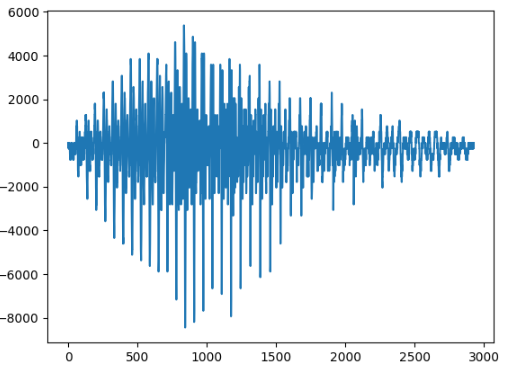
\includegraphics[width=10cm]{./capture/spoken_digit_1.png}
  \caption{Spoken Degitで取得したある音声データ波形}
  \label{fig:Spoken_Degit}
\end{figure}

TensorFlowにはmap関数が用意されており、データセットに対して関数を適用することができる。例えば、
\begin{itembox}[l]{}
\begin{verbatim}
  def normalize(example):
    audio = example['audio']
    audio = audio / tf.reduce_max(audio)
    return {'audio': audio, 'label': example['label']}

  dataset_train = dataset_train.map(normalize)
\end{verbatim}
\end{itembox}
のように、normalize関数を定義し、map関数を用いてデータセットに適用することができる。この場合、音声データを正規化している。

map関数を用いて、教師ラベルと音声データをペアで用意したものを用いて、TensorFlowのKeras APIを使ってLSTMで0から9までの数字を予測するモデルを構築する場合、以下の手順を経る。
\begin{enumerate}
  \item データセットの準備 (上述のようにデータセットを用意する)
  \item モデルの構築 (model = tf.keras.models.Sequential())
  \item レイヤーの追加 (model.add(layers.Input), model.add(layers.LSTM), model.add(layers.Dense))
  \item モデルのコンパイル (model.compile())
  \item モデルの学習 (model.fit())
  \item モデルの評価 (model.evaluate())
\end{enumerate}
  
評価には、テストデータを正しく予測できているか目で確認してみることも大切である。その際には、
\begin{itembox}[l]{}
\begin{verbatim}
  predictions = model.predict(dataset_test)
  print(predictions[0])
  print('予測: ', np.argmax(predictions[0]))
  print('正解: ', dataset_test[1][0])
\end{verbatim}
\end{itembox}
とすると、予測と正解が表示できる。


\subsection{Data Augmentation}
Data Augmentationは、データの水増しを行う手法である。データの水増しは、データセットのサイズを増やすことで、過学習を防ぐ効果がある。Data Augmentationの手法としては、Horizontal Flip (水平方向の反転処理), Vertical Flip (垂直方向の反転処理), Random Crop (ランダムに切り取る処理), 
Random Rotation (ランダムに回転させる処理), Contrast (コントラスト), Brightness (明るさ), Hue (色相)などがある。
\par
また、TensorFlowには、Random Erasing(ランダムにマスクする処理), Mixup(2つの画像を混ぜ合わせる処理), CutMix(画像の一部を切り取り、貼り付ける処理)などのData Augmentationの手法が用意されている。
\par
これらの手法を組み合わせて用いることで、合計で100倍程度のデータセットを用意することができる。これによって、過学習を防ぐことができる。

\paragraph{参考文献}
\begin{enumerate}
  \item 岡谷貴之/深層学習 改訂第2版 [機械学習プロフェッショナルシリーズ]/ 講談社サイエンティフィク/ 2022-01-17
  \item RNN入門PART1$\sim$3/@\_livesomewhere1090 \url{https://www.youtube.com/@\_livesomewhere1090}
  \item 絵で理解するWord2vecの仕組み \url{https://qiita.com/Hironsan/items/11b388575a058dc8a46a}
  \item TensorFlow, Kerasの基本的な使い方(モデル構築・訓練・評価・予測)\url{https://note.nkmk.me/python-tensorflow-keras-basics/}
\end{enumerate}

\end{document}